\section{Теория кривых}

\epigraph{Рубины шлифуют алмазами.}{А.\,А. Гайфуллин}

\subsection{Базовые определения}

\begin{definition}
	\textit{Простой дугой} $\gamma$ в $\R^n$ называется любое подмножество $\R^n$, гомеоморфное отрезку $[0; 1]$. \textit{Параметризацией} простой дуги называется гомеоморфизм $\vec{r}\colon [0; 1] \to \gamma$.
\end{definition}

\begin{definition}
	Параметризация $\vec{r}\colon [0; 1] \to \R^n$ простой дуги называется \textit{регулярной класса $C^k$}, если для всех $i = 1, \ldots, n$ функция $r^i(t)$ является отображением класса $C^k$ и
	\[
		\frac{d\vec{r}}{dt} > 0
	\]
	в каждой точке (для концов отрезка $0$ и $1$ в качестве производной берётся производная справа и слева соответственно). Простая дуга называется \textit{регулярной} (или \textit{гладкой}), если существует её регулярная параметризация.
\end{definition}

Параметризация простой дуги естественным образом задаёт на ней ориентацию. Условие на знак производной в данной точке необходимо, чтобы сохранять эту ориентацию при замене параметра.

\begin{definition}
	\textit{Параметризованной кривой} в $\R^n$ называется непрерывное отображение $\vec{r}\colon I \to \R$ такое, что существует не более чем счётное покрытие промежутка $I$ отрезками $[a_i; b_i]$ такое, что для каждого $i$ ограничение $\left.\vec{r}\right|_{[a_i; b_i]}$ есть параметризация простой дуги.
\end{definition}

\begin{definition}
	\textit{Кривой} в $\R^n$ называется класс эквивалентности параметризованных кривых, где $\vec{r}_1\colon I_1 \to \R^n$ и $\vec{r}_2\colon I_2 \to \R^n$ \textit{эквивалентны}, если существует такой гомеоморфизм $I_1 \to I_2$, что следующая диаграмма коммутативна:
	\shorthandoff{"}%
	\begin{equation*}
		\begin{tikzcd}
			I_1 && {\R^n} \\
			\\
			I_2 && {\R^n}
			\arrow["\vec{r}_1", hook, from=1-1, to=1-3]
			\arrow["\cong"', from=1-1, to=3-1]
			\arrow["\id", from=1-3, to=3-3]
			\arrow["\vec{r}_2", hook, from=3-1, to=3-3]
		\end{tikzcd}
	\end{equation*}
	\shorthandon{"}%
	Любое вложение из данного класса будем называть \textit{параметризацией} кривой.
\end{definition}

В дальнейшем мы будем рассматривать только регулярные кривые. Условие регулярности необходимо добавить для соответствия интуитивному пониманию гладкости как отсутствия изломов.
\begin{figure}[h]
	\centering
	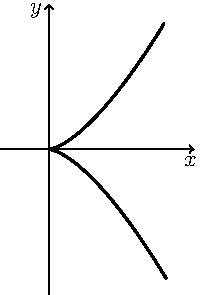
\includegraphics[height=5cm]{./img/SemicubicalParabola.pdf}
	\caption{Полукубическая парабола}
	\label{fig:SemicubicalParabola}
\end{figure}
Например, мы не хотим рассматривать кривые вроде $\vec{r}(t) = (t^2, t^3)$ (рис. \ref{fig:SemicubicalParabola}), хотя обе координатные функции $x(t) = t^2$ и $y(t) = t^3$ гладкие класса $C^\infty$.

\begin{proposition} \label{proposition:SmoothHomeomorphism}
	Если $\vec{r}_1(t)$ и $\vec{r}_2(s)$ --- регулярные эквивалентные параметризации, то $t(s)$ и $s(t)$ являются гладкими функциями.
\end{proposition}

\begin{proof}
	Рассмотрим параметр $t$. Так как обе параметризации регулярны, то $\dot{\vec{r}}_1(t_0) \ne 0$ в каждой точке $t_0$. Тогда найдётся номер $i_0$ такой, что $\dot{x}^{i_0}(t_0) \ne 0$. Тогда по теореме об обратной функции в некоторой окрестности точки $t_0$ можно выразить параметр $t$ через $x^{i_0}$, то есть $t(x^{i_0})$ --- гладкая функция в некоторой окрестности данной точки. А $x^{i_0}$, в свою очередь, является гладкой функцией от $s$ (так как отображение $\vec{r}_2$ гладкое). Таким образом, функция $t(s) = t(x^{i_0}(s))$ гладкая как композиция гладких функций (теорема о сложной функции). Аналогично доказывается, что функция $s(t)$ тоже гладкая.
\end{proof}

Важно подчеркнуть, что при доказательстве использовалось рассуждение, которое можно сформулировать так: на регулярной кривой в некоторой окрестности любой точки можно в качестве параметра выбрать одну из координат евклидова пространства. Отсюда, например, можно сразу получить нерегулярность полукубической параболы --- легко видеть, что в окрестности точки $(0, 0)$ её нельзя параметризовать ни одной переменной $x$ или $y$.

\subsection{Способы задания кривой}

На практике часто приходится иметь дело с кривыми, заданными с помощью уравнений. С глобальной точки зрения данный подход не эквивалентнен параметрическому заданию. Однако, если наложить на систему уравнений некоторые ограничения, то мы получим объекты, локально устроенные так же, как кривые.

\begin{definition}
	Пусть $\vec{f}$ --- гладкая функция из некоторого подмножества $U \subset \R^n$ в $\R^m$, $m \leqslant n$. Мы говорим, что точка $\vec{x}_0 \in U$ является для неё \textit{регулярной}, если $\vec{x}_0 \in \Int U$ и $\rk J_{\vec{f}}(\vec{x}_0) = m$.
\end{definition}

\begin{theorem} \label{theorem:SurfacesToCurve}
	Пусть $f_1, \ldots, f_{n - 1}$ --- набор гладких функций из некоторого подмножества $U \subset \R^n$ в $\R$, а точка $\vec{x}_0 \in U$ является регулярной точкой отображения $\vec{f} = (f_1, \ldots, f_{n - 1})$ и решением системы уравнений
	\[
		\begin{cases}
			f_1(\vec{x}) = 0,\\
			\dotfill\\
			f_{n - 1}(\vec{x}) = 0,
		\end{cases}
	\]
	то есть $\vec{f}(\vec{x}_0) = \vec{0}$. Тогда существует окрестность точки $\vec{x}_0$, в которой пространство решений этой системы представляет собой гладкую регулярную кривую.
	
	Верно и обратное: в окрестности любой точки регулярной кривой её можно задать системой уравнений, которая регулярна в этой точке.
\end{theorem}

\begin{proof}
	Без ограничения общности, можем считать, что первые $n - 1$ столбцов матрицы $J_{\vec{f}}(\vec{x}_0)$ линейно независимы (иначе перенумеруем координаты). Тогда по теореме о неявной функции решение этой системы в некоторой окрестности точки $\vec{x}_0$ задаётся гладкими функциями $x^1(x^n), \ldots, x^{n - 1}(x^n)$. Но это и означает, что локально решения представляют собой регулярную кривую, так как радиус-вектор параметризован последней координатой: $\vec{r}(x^n) = (x^1(x^n), \ldots, x^{n - 1}(x^n), x^n)$. Эта параметризация регулярна, поскольку последней компонентой вектора скорости $\dot{\vec{r}}$ будет $1$.

	Докажем обратное утверждение. Как упоминалось в предложении \ref{proposition:SmoothHomeomorphism}, в качестве параметра локально можно взять одну из координат. Не теряя общности, будем считать, что эта координата $x^n$: $\vec{r}(x^n) = (x^1(x^n), \ldots, x^{n - 1}(x^n), x^n)$. Теперь запишем систему уравнений $\vec{x} - \vec{r}(x^n) = \vec{0}$, которая локально задаёт нашу кривую. Первые $n - 1$ столбец матрицы Якоби $J_{\vec{x} - \vec{r}(x^n)}$ в рассматриваемой точке составляют единичную матрицу.
\end{proof}

\subsection{Касательная в точке регулярной кривой}

\begin{definition}
	Пусть регулярная кривая задана радиус-вектором $\vec{r}(t)$. \textit{Касательная прямая} к этой кривой в точке $t_0$ задаётся рядом Тейлора функции $\vec{r}$ с отбрасыванием всех членов более высокого порядка, чем $t - t_0$:
	\[
		\vec{\ell}(t) \vcentcolon = \vec{r}(t_0) + \left.\frac{d\vec{r}}{dt}\right|_{t_0}(t - t_0).
	\]
\end{definition}

Нужно проверить корректность данного определения, ведь оно сформулировано для конкретной параметризации кривой. Здесь корректность сразу следует из предложения \ref{proposition:SmoothHomeomorphism} и теоремы о сложной функции:
\[
	\frac{d\vec{r}}{dt} = \frac{d\vec{r}}{ds} \frac{ds}{dt}.
\]

\begin{theorem}
	\begin{enumerate}[nolistsep, label=(\arabic*)]
		\item Пусть $\gamma$ --- регулярная кривая, $\vec{x}_0 \in \gamma$ --- некоторая её точка, $\ell$ --- касательная прямая в точке $\vec{x}$. Тогда для $\vec{x}_1 \in \gamma$, $\vec{x}_1 \ne \vec{x}_0$ выполнено
			\[
				\rho(\vec{x}_1, \ell) = \o(\abs{\vec{x}_1 - \vec{x}_0})\text{ при $\vec{x}_1 \to \vec{x}_0$}.
			\]
		\item Для каждой точки $\vec{x}_0 \in \gamma$ касательная прямая является единственной прямой с указанным свойством.
	\end{enumerate}
\end{theorem}

\begin{proof}
	Пусть на $\gamma$ выбрана регулярная параметризация $\vec{r}(t)$, в которой $\vec{x}_0 \hm= \vec{r}(0)$. В качестве точки $\vec{x}_1$ будем брать $\vec{r}(t)$, где $t$ пробегает окрестность нуля. Условие $\vec{r}(t) \to \vec{x}_0$ можно заменить на $t \to 0$ (по определению кривой). Обозначим $\vec{v}_0 \vcentcolon = \dot{\vec{r}}(0)$. По условию, $\vec{v}_0 \ne 0$.
	\begin{enumerate}[nolistsep, label=(\arabic*)]
		\item По формуле Тейлора имеем
			\[
				\vec{r}(t) = \vec{x}_0 + \vec{v}_0t + \o(t) = \vec{x}_0 + (\vec{v}_0 + \o(1))t\text{ при $t \to 0$}.
			\]
			Расстояние от $\vec{r}(t)$ до прямой $\ell$ равно $\rho(\vec{r}(t), \ell) = \abs{\vec{r}(t) - \vec{x}_0}\sin\alpha(t)$, где $\alpha(t)$ --- угол между векторами $\vec{v}_0$ и $\vec{r}(t) - \vec{x}_0$. Поскольку $\vec{r}(t) - \vec{x}_0 = (\vec{v}_0 + \o(1))t$, этот угол равен $\o(1)$ при $t \to 0$. Получаем
			\[
				\rho(\vec{r}(t), \ell) = \abs{\vec{r}(t) - \vec{x}_0}\o(1) = \o(\abs{\vec{r}(t) - \vec{x}_0}).
			\]
			\begin{figure}[H]
				\centering
				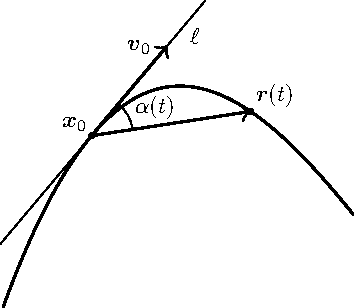
\includegraphics[width=6cm]{./img/Curve.pdf}
				\caption[format=empty]{}
			\end{figure}
		\item Пусть теперь $\ell^\prime$ --- другая прямая, проходящая через точку $\vec{x}_0$, и пусть $\vec{u}$ --- её направляющий вектор. Тогда
			\[
				\rho(\vec{r}(t), \ell^\prime) = \abs{\vec{r}(t) - \vec{x}_0}\sin\beta(t),
			\]
			где $\beta(t)$ --- угол между векторами $\vec{u}$ и $\vec{r}(t) - \vec{x}_0 = (\vec{v}_0 + \o(1))t$. При $t \to 0$ угол $\beta(t)$ стремится к углу между векторами $\vec{u}$ и $\vec{v}_0$, который по предположению отличен от $0$ и $\pi$. Отсюда $\rho(\vec{r}(t), \ell^\prime) = \abs{\vec{r}(t) - \vec{x}_0}(\const + \o(1))$, где $\const \ne 0$.
	\end{enumerate}
\end{proof}

\begin{proposition}
	Если кривая в $\R^n$ задана системой уравнений $\vec{f}(\vec{x}) = \vec{0}$, то касательная к ней в регулярной точке $\vec{x}_0$ задаётся системой уравнений $J_{\vec{f}}(\vec{x}_0) \cdot (\vec{x} - \vec{x}_0) = 0$.
\end{proposition}

\begin{proof}
	Точка $\vec{x}_0$ регулярна для отображения $\vec{f}$, значит, $\rk J_{\vec{f}}(\vec{x}_0) = n - 1$, поэтому пространство решений системы с этой матрицей одномерно, то есть задаёт прямую в пространстве $\R^n$ (очевидно, проходящую через точку $\vec{x}_0$). Остаётся проверить, что эта прямая параллельна вектору скорости касательной прямой в точке $\vec{x}_0$.

	Пусть $\vec{r}(t)$ --- регулярная параметризация данной кривой в окрестности точки $\vec{x}_0 \hm= \vec{r}(t_0)$ (существует по теореме \ref{theorem:SurfacesToCurve}). Это означает, что $\vec{f}(\vec{r}(t)) = 0$ для всех $t$ из прообраза данной окрестности. По теореме о производной сложной функции имеет место равенство
	\[
		\frac{d}{dt}\vec{f}(\vec{r}(t)) = \left.\frac{\partial\vec{f}}{\partial\vec{x}}\right|_{\vec{r}(t)}\dot{\vec{r}}(t).
	\]
	Подставляя $t = t_0$, получаем
	\[
		\left.\frac{\partial\vec{f}}{\partial\vec{x}}\right|_{\vec{x}_0}\vec{v}_0 = 0,
	\]
	где $\vec{v}_0$ --- вектор скорости при $t = t_0$.
\end{proof}

\subsection{Натуральный параметр и кривизна}

\begin{definition}
	\textit{Длиной} кривой, заметаемой при изменении значения параметра от $t_0$ до $t$, называется число
	\[
		l = \int\limits_{t_0}^t\abs{\dot{\vec{r}}(t)}dt.
	\]
\end{definition}

Здесь опять нужно проверить корректность, то есть независимость от параметризации. Пусть мы перешли к другому регулярному параметру $s$ (причём $dt / ds > 0$). Тогда имеем
\[
	\int\limits_{s_0}^s\abs{\frac{d\vec{r}}{ds}}ds = \int\limits_{t_0}^t\abs{\frac{d\vec{r}}{dt}\frac{dt}{ds}}\frac{ds}{dt}dt = \int\limits_{t_0}^t\abs{\frac{d\vec{r}}{dt}}\frac{\cancel{dt}}{\cancel{ds}}\frac{\cancel{ds}}{\cancel{dt}}dt = \int\limits_{t_0}^t\abs{\frac{d\vec{r}}{dt}}dt = l.
\]

\begin{definition}
	Параметр $s$ называется \textit{натуральным параметром} регулярной кривой, если $\abs{d\vec{r} / ds} = 1$.
\end{definition}

\begin{proposition} \label{proposition:LengthParameter}
	\begin{enumerate}[nolistsep, label=(\arabic*)]
		\item Длина кривой $l(t)$ является натуральным параметром.
		\item Если $s$ --- некоторый натуральный параметр, то $s = l + \const$.
	\end{enumerate}
\end{proposition}

\begin{proof}
	\begin{enumerate}[nolistsep, label=(\arabic*)]
		\item $dl / dt = \abs{d\vec{r} / dt} > 0$. Значит, по теореме об обратной функции можем локально выразить $t = t(l)$, и при этом
			\[
				\abs{\frac{d\vec{r}}{dl}} = \abs{\frac{d\vec{r}}{dt}\frac{dt}{dl}} = \frac{dt}{dl}\abs{\frac{d\vec{r}}{dt}} = \frac{\abs{d\vec{r} / dt}}{\abs{d\vec{r} / dt}} = 1.
			\]
		\item Если $s$ --- натуральный параметр, то $\abs{\dot{\vec{r}}(s)} = 1$ для каждого $s$. Отсюда,
			\[
				l(s) = \int\limits_{s_0}^s\abs{\dot{\vec{r}}(s)}ds = s - s_0,
			\]
			то есть $s = l + s_0$, что и требовалось.
	\end{enumerate}
\end{proof}

Далее, если не указано иное, через $s$ мы будем всегда обозначать натуральный параметр, а через $\dot{\vec{r}}$ --- производную по натуральному параметру.

Предложение \ref{proposition:LengthParameter} говорит нам о том, что натуральный параметр на любой кривой можно выписать явно по формуле длины кривой. Наличие такой формулы говорит нам о том, что у кривых тривиальная внутренняя геометрия. Всё, что можно делать на кривой --- мерять длины, и мы (теоретически) можем это делать в любой параметризации.

\begin{definition}
	\textit{Кривизной} кривой в точке $s$ называется величина $k(s) \vcentcolon = \abs{\ddot{\vec{r}}(s)}$. (Легко видеть, что кривизна не зависит от выбора натурального параметра $s$.)
\end{definition}

\begin{proposition}
	Кривизна регулярной кривой на некотором участке равна нулю тогда и только тогда, когда этот участок является частью прямой.
\end{proposition}

\begin{proof}
	$\Rightarrow$. Если $k(s) = 0$, то $\ddot{\vec{r}}(s) = 0$. Тогда $\vec{r}(s)$ должен быть линеен по $s$, то есть быть уравнением прямой.

	$\Leftarrow$. Рассмотрим прямую $\vec{r}(t) = \vec{x}_0 + \vec{v}t$. Перейдём к натуральному параметру, воспользовавшись результатами предложения \ref{proposition:LengthParameter}:
	\[
		s(t) = \int\limits_0^t\abs{\dot{\vec{r}}(t)}dt = \int\limits_0^t \abs{\vec{v}}dt = \abs{\vec{v}}t.
	\]
	Подставляя найденное, легко убеждаемся, что $\vec{r}(s)$ линейно, значит, $\ddot{\vec{r}}(s) = 0$.
\end{proof}

Результат последнего предложения согласуется с нашим интуитивным представлением о кривизне --- кривизна прямой должна быть равна нулю, а чего-то кроме прямой --- не равна нулю.

\begin{definition}
	Регулярная кривая называется \textit{бирегулярной} на некотором интервале, если кривизна не равна нулю на этом интервале.
\end{definition}

Полезно также посчитать кривизну окружности. В натуральном параметре уравнение окружности радиуса $R$ имеет следующий вид:
\[
	\vec{r}(s) = \br{R\cos\frac{s}{R}, R\sin\frac{s}{R}}
\]

Кривизна равна $k(s) = \abs{\ddot{r}(s)} = \frac{1}{R}$, что тоже соответствует нашему интуитивному представлению: кривизна окружности во всех точках одинакова и уменьшается с увеличением радиуса.

В натуральном параметре $\abs{\dot{\vec{r}}(s)} = 1$, значит, $\dot{\vec{r}}(s) \perp \ddot{\vec{r}}(s) = 0$. Таким образом, в каждой точке $\vec{r}(s)$ кривой имеем свой ортонормированный базис из вектора скорости $\vec{v}(s) \vcentcolon = \dot{\vec{r}}(s)$ и вектора \textit{главной нормали} $\vec{n}(s) \vcentcolon = \ddot{\vec{r}}(s) / \abs{\ddot{\vec{r}}(s)}$. (Для корректности этого определения считаем кривую бирегулярной.) Плоскость $\span(\vec{v}(s), \vec{n}(s))$ называется \textit{соприкасающейся плоскостью} кривой в точке $s$.

\begin{proposition} \label{proposition:TouchPlane}
	В любой параметризации линейная оболочка векторов скорости и ускорения лежит в соприкасающейся плоскости.
\end{proposition}

\begin{proof}
	Перейдём от некоторого регулярного параметра $t$ к натуральному параметру $s$:
	\[
		\frac{d\vec{r}(t)}{dt} = \frac{d\vec{r}(s)}{ds} \frac{ds}{dt},\quad \frac{d^2\vec{r}(s)}{ds^2} = \frac{d^2\vec{r}(s)}{ds^2}\br{\frac{ds}{dt}}^2 + \frac{d\vec{r}(s)}{ds}\frac{d^2s}{dt^2}.
	\]

	Из первой формулы видно, что все вектора скорости коллинеарны, а из второй --- что вектор ускорения в любой регулярной параметризации является линейной комбинацией векторов скорости и ускорения в натуральной параметризации и, как следствие, принадлежит соприкасающейся плоскости.
\end{proof}

Выведем формулу кривизны в произвольной параметризации. Заметим, что
\[
	\abs{S_{\Or}(\dot{\vec{r}}(s), \ddot{\vec{r}}(s))} = k(s) \cdot \underbrace{\abs{S_{\Or}(\vec{v}(s), \vec{n}(s))}}_1 = k(s).
\]

Теперь выразим производные по $s$ через произвольный параметр $t$ (производные по $t$ будем обозначать штрихом). Сразу из определения натурального параметра имеем $\frac{ds}{dt} \hm= \abs{\vec{r}^\prime(t)}$, $\dot{\vec{r}}(s) = \vec{r}^\prime(t) / \abs{\vec{r}^\prime(t)}$. Считаем вторую производную:
\[
	\ddot{\vec{r}}(s) = \frac{d}{ds}\br{\frac{\vec{r}^\prime(t)}{\abs{\vec{r}^\prime(t)}}} = \br{\frac{\vec{r}^\prime(t)}{\abs{\vec{r}^\prime(t)}}}^\prime \frac{dt}{ds} = \frac{\vec{r}^{\prime\prime}(t) \abs{\vec{r}^\prime(t)} - \vec{r}^\prime(t)\frac{d}{dt}\abs{\vec{r}^\prime(t)}}{\abs{\vec{r}^\prime(t)}^3} = \frac{\vec{r}^{\prime\prime}(t)}{\abs{\vec{r}^\prime(t)}^2} - \frac{\frac{d}{dt}\abs{\vec{r}^\prime(t)}}{\abs{\vec{r}^\prime(t)}^3}\vec{r}^\prime(t).
\]
Подставляем в формулу, выведенную для натуральной параметризации:
\begin{equation} \label{eq:CurvatureFormula}
	k(t) = \abs{S_{\Or}(\dot{\vec{r}}(s), \ddot{\vec{r}}(s))} = \abs{S_{\Or}\br{\frac{\vec{r}^\prime(t)}{\abs{\vec{r}^\prime(t)}}, \frac{\vec{r}^{\prime\prime}(t)}{\abs{\vec{r}^{\prime}(t)}^2}}} = \frac{\abs{S_{\Or}(\vec{r}^\prime(t), \vec{r}^{\prime\prime}(t))}}{\abs{\vec{r}^\prime(t)}^3}.
\end{equation}

Смогли отбросить второе слагаемое в выражении $\vec{r}^{\prime\prime}(s)$, так как вектор в этом слагаемом был коллинеарен $\vec{r}^\prime(t)$, поэтому при подстановке в ориентированную площадь давал $0$.

\subsection{Соприкасающаяся окружность}

\begin{definition}
	Говорят, что две гладкие кривые \textit{имеют в точке $\vec{x}_0$ соприкосновение порядка $k$}, где $k \geqslant 1$, если для некоторых их регулярных параметризаций и некоторого $t_0$ выполнено
	\begin{equation} \label{eq:OsculatingCurve}
		\vec{r}_1(t_0) = \vec{r}_2(t_0) = \vec{x}_0,\quad\abs{\vec{r}_1(t) - \vec{r}_2(t)} = \o((t - t_0)^k)\text{ при $t \to t_0$}.
	\end{equation}
\end{definition}

Из формулы Тейлора следует, что условие \eqref{eq:OsculatingCurve} равносильно следующему:
\[
	\vec{r}_1 = \vec{r}_2(t_0),\quad \vec{r}_1^\prime(t_0) = \vec{r}_2^\prime(t_0),\quad \ldots,\quad \br{\frac{d^k\vec{r}_1}{dt^k}}(t_0) = \br{\frac{d^k\vec{r}_2}{dt^k}}(t_0).
\]

Касательная прямая к кривой имеет в точке касания первый порядок соприкосновения с этой кривой. Однако может иметь и больший порядок соприкосновения.

\begin{definition}
	Точка $\vec{x}$ кривой $\gamma$ называется \textit{точкой спрямления}, если в ней кривая $\gamma$ имеет со своей касательной прямой соприкосновение порядка два.
\end{definition}

\begin{proposition} \label{proposition:Inflection}
	Пусть дана кривая с регулярной парамеризацией $\vec{r}(t)$. Точка, соответствующая значению параметра $t = t_0$ является точкой спрямления тогда и только тогда, когда векторы скорости $\vec{r}^\prime(t_0)$ и $\vec{r}^{\prime\prime}(t_0)$ коллинеарны.
\end{proposition}

\begin{proof}
	$\Rightarrow$. Пусть $\vec{\ell}(t)$ --- параметризация касательной в точке спрямления. Тогда имеем $\vec{r}^\prime(t) = \vec{\ell}^\prime(t)$ и $\vec{r}^{\prime\prime}(t) = \vec{\ell}^{\prime\prime}(t)$, а вектора $\vec{\ell}^\prime$ и $\vec{\ell}^{\prime\prime}$ коллинеарны, так как они сонаправлены одной и той же касательной прямой.

	$\Leftarrow$. Параметризуем отрезок касательной прямой возле точки $\vec{r}(t_0)$ следующим образом:
	\[
		\vec{\ell}(t_0) = \vec{r}(t_0) + \vec{r}^\prime(t_0)t + \frac{\vec{r}^{\prime\prime}(t_0)}{2}t^2,\ t \in [t_0 - \eps; t_0 + \eps].
	\]
	При достаточно малом $\eps$ эта параметризация регулярна, так как $\vec{r}^{\prime}(t_0) \ne 0$.
\end{proof}

Отметим, что точки спрямления --- ровно те точки кривой, в которых её кривизна равна нулю. Действительно, в натуральной параметризации $\abs{\dot{\vec{r}}} = 1$, так что $\dot{\vec{r}} \perp \ddot{\vec{r}}$, но в точках спрямления $\dot{\vec{r}} \parallel \ddot{\vec{r}}$. Так что остаётся единственная возможность $\ddot{\vec{r}} = \vec{0}$.

\begin{theorem}
	Пусть $\gamma_1$ и $\gamma_2$ --- две гладкие простые дуги в $\R^n$, имеющие общую точку $\vec{x}_0$. Они имеют в этой точке соприкосновение порядка $k$ тогда и только тогда, когда для $\vec{x} \in \gamma_1$ выполнено
	\begin{equation} \label{eq:rhoo}
		\rho(\vec{x}, \gamma_2) = \o(\abs{\vec{x} - \vec{x}_0}^k)\text{ при $\vec{x} \to \vec{x}_0$}.
	\end{equation}
\end{theorem}

\begin{proof}
	Пусть $\vec{r}_1$ и $\vec{r}_2$ --- регулярные параметризации данных кривых такие, что $\vec{r}_1(0) = \vec{r}_2(0) = \vec{x}_0$.

	$\Rightarrow$. Без ограничения общности можно считать, что $\dot{\vec{r}}_1(0) \parallel \vec{e}_1$. Тогда за параметр на $\gamma_1$ можно выбрать первую координату, то есть
	\[
		\vec{r}_1(t) = \vec{x_0} + (t, \o(t), \ldots, \o(t)),\,t \to 0.
	\]
	Для такой параметризации имеем
	\[
		\abs{\vec{r}_1(t) - \vec{x}_0} = (1 + \o(1))\abs{t},\,t \to 0,
	\]
	то есть величины $\abs{\vec{r}_1(t) - \vec{x}_0}$ и $t$ одного порядка малости при $t \to 0$, и можно заменять $\o(\abs{\vec{r}_1(t) - \vec{x}_0}^k)$ на $\o(t^k)$, и наоборот. Отсюда, условие \eqref{eq:OsculatingCurve} влечёт \eqref{eq:rhoo}.

	Пусть выполнено \eqref{eq:rhoo}. Обозначим через $\varphi(t)$ функцию, определённую в окрестности $0$ условием
	\[
		\abs{\vec{r}_1(t) - \vec{r}_2(\varphi(t))} = \o(\abs{\vec{r}_1(t) - \vec{x}_0}^k).
	\]
	(Мы не требуем от $\varphi$ гладкости и даже непрерывности. В качестве $\varphi(t)$ можно взять параметр, соответствующий точек кривой $\vec{r}_2$, на которой достигается расстояние от точки $\vec{r}_1(t)$ до кривой $\vec{r}_2$.) Из определения простой дуги следует, что $\varphi(t) \to 0$ при $t \to 0$. Кроме того, направление вектора $\vec{r}_2(\varphi(t)) - \vec{x}_0$ (рассматриваемое с точностью до знака) стремится к направлению вектора $\dot{\vec{r}}_1(0) = (1, 0, \ldots, 0)$, а значит, первую координату можно взять за параметр и на второй дуге.

	С этого места мы предполагаем, что параметризация второй дуги также имеет вид
	\[
		\vec{r}_2(t) = \vec{x}_0 + (t, \o(t), \ldots, \o(t)),\,t \to 0.
	\]

	Рассмотрим треугольник с вершинами $\vec{x} = \vec{r}_1(t)$, $\vec{x}_1 = \vec{r}_2(t)$, $\vec{x}_2 = \vec{r}_2(\varphi(t))$ при $t \hm\to 0$. Направление вектора $\vec{x}_2 - \vec{x}_1$, если он ненулевой, сближается с направлением вектора скорости второй кривой в точке $\vec{x}_0$, то есть $\vec{v}_0 = (1, 0, \ldots, 0)$. При этом $(\vec{x}_1 - \vec{x}) \perp \vec{v}_0$. Таким образом, угол $\angle \vec{x}\vec{x}_1\vec{x}_2$ стремится к прямому. Мы знаем, что противолежащая ему сторона $\vec{x}\vec{x}_2$ имеет порядок малости $\o(\abs{\vec{x} - \vec{x}_0}^k) = \o(t^k)$. Отсюда, все его стороны имеют по крайней мере такой же порядок малости, в частности, $\abs{\vec{x} - \vec{x}_1} = \abs{\vec{r}_1(t) - \vec{r}_2(t)}$, откуда следует $\eqref{eq:OsculatingCurve}$.
\end{proof} % TODO: картинку!

\begin{definition}
	\textit{Соприкасающейся окружностью} с данной кривой $\vec{r}(t)$ в точке $\vec{x}_0$ называется окружность, которая имеет соприкосновение второго порядка с этой кривой в точке $\vec{x}_0$.
\end{definition}

\begin{theorem} \label{theorem:TouchingCircle}
	Если точка $\vec{x}_0$ некоторой гладкой кривой $\gamma$ не является точкой спрямления, то существует ровно одна окружность, имеющая в $\vec{x}_0$ соприкосновение второго порядка с~$\gamma$.
\end{theorem}

\begin{proof}
	Пусть $\vec{r}(t)$ --- некоторая регулярная параметризация кривой $\gamma$ с условием $\vec{r}(0) = \vec{x}_0$. Соприкосновение второго порядка в точке $\vec{x}_0$ с какой-либо другой кривой определяется векторами скорости $\vec{v} = \dot{\vec{r}}(0)$ и ускорения $\vec{a} = \ddot{\vec{r}}(0)$. Поэтому для доказательства теоремы достаточно взять любую другую кривую с теми же векторами скорости и ускорения в точке $\vec{x}_0$. Таким образом, без ограничения общности мы можем считать, что наша кривая имеет следующую параметризацию:
	\[
		\vec{r}(t) = \vec{x}_0 + \vec{v}t + \frac{\vec{a}}{2}t^2.
	\]
	Так как $\vec{x}_0$ --- не точка спрямления, векторы $\vec{v}$ и $\vec{a}$ линейно независимы (см. предложение \ref{proposition:Inflection}), и порождают соприкасающуюся плоскость (см. предложение \ref{proposition:TouchPlane}).

	Пусть $C$ --- окружность, проходящая через $\vec{x}_0$. При любой её параметризации векторы скорости и ускорения лежат в той же плоскости, что и она сама. Поэтому необходимым условием соприкосновения окружности $C$ с кривой $\gamma$ в точке $\vec{x}_0$ является то, что эта окружность лежит в соприкасающейся плоскости $\span(\vec{v}, \vec{a})$, что мы дальше и предполагаем.

	Пусть $O$ --- центр окружности $C$. Тогда вектор $\vec{u} = \overrightarrow{O\vec{x}_0}$ является линейной комбинацией векторов $\vec{v}$ и $\vec{a}$: $\vec{u} = \lambda\vec{v} + \mu\vec{a}$. Расстояние от произвольной точки $\vec{x} \in \span(\vec{v}, \vec{a})$ до $C$ равно
	\[
		\rho(\vec{x}, C) = \Big\lvert\big\lvert\overrightarrow{O\vec{x}}\big\rvert - R\Big\rvert,
	\]
	где $R$ --- радиус окружности $C$. Отсюда условие соприкосновения окружности $C$ и кривой $\gamma$ можно записать так:
	\[
		\big\lvert\overrightarrow{O\vec{r}(t)}\big\rvert - R = \o(t^2),
	\]
	что равносильно (поскольку $R \ne 0$)
	\[
		\big\lvert\overrightarrow{O\vec{r}(t)}\big\rvert^2 = R^2 + \o(t^2).
	\]
	Подставляя $\overrightarrow{O\vec{r}(t)} = \vec{u} + \vec{v}t + \frac{\vec{a}}{2}t^2$, получаем
	\[
		\left\langle\vec{u} + \vec{v}t + \frac{\vec{a}}{2}t^2, \vec{u} + \vec{v}t + \frac{\vec{a}}{2}t^2\right\rangle = R^2 + \o(t^2).
	\]
	Раскрывая скобки в левой части и отбрасывая члены порядка $\o(t^2)$, получаем
	\[
		\langle\vec{u}, \vec{u}\rangle + 2\langle\vec{u}, \vec{v}\rangle t + (\langle\vec{u}, \vec{a}\rangle + \langle\vec{v}, \vec{v}\rangle)t^2 = R^2.
	\]
	Учитывая равенство $R = \abs{\vec{u}}$, мы приходим к следующему условию соприкосновения второго порядка окружности $C$ и кривой $\gamma$:
	\[
		\langle\vec{u}, \vec{v}\rangle = 0,\quad \langle\vec{u}, \vec{a}\rangle + \langle\vec{v}, \vec{v}\rangle = 0.
	\]
	Подставляя $\vec{u} = \lambda\vec{v} + \mu\vec{a}$, получаем систему линейных уравнений на $\lambda$ и $\mu$:
	\[
		\br{
			\begin{array}{cc | c}
				\langle\vec{v}, \vec{v}\rangle & \langle\vec{v}, \vec{a}\rangle & 0\\
				\langle\vec{a}, \vec{v}\rangle & \langle\vec{a}, \vec{a}\rangle & -\langle\vec{v}, \vec{v}\rangle
			\end{array}
		},
	\]
	матрица которой есть матрица Грама векторов $(\vec{v}, \vec{a})$, которая невырождена из линейной независимости этих векторов, так что система имеет единственное решение.
\end{proof}

Соприкосновение кривых второго (или более) порядка влечёт равенство кривизн кривых в точке соприкосновения. Значит, радиус соприкасающейся окружности равен $R = 1 / k$, где $k$ --- кривизна в точке соприкосновения. Таким образом, соприкасающаяся окружность даёт геометрический смысл понятия кривизны, так что её центр часто называют \textit{центром кривизны}, а радиус --- \textit{радиусом кривизны}.

\subsection{Кривые на плоскости и в пространстве}

Далее считаем, что задана плоская кривая $\gamma$ с натуральной параметризацией $\vec{r}(s)$.

\begin{definition}
	Точку $\vec{r}(s)$ и приложенный к ней базис $(\vec{v}(s), \vec{n}(s))$ называют \textit{репером Френе} плоской кривой.
\end{definition}

В каждой точке кривой введён свой локальный базис. Поэтому и векторы, связанные с точками на кривых, будут задаваться в этих локальных базисах. Чтобы дифференцировать такие векторы, нам нужно научиться дифференцировать векторы $\vec{v}$ и $\vec{n}$.

\begin{theorem}[\textit{Формулы Френе для плоской кривой}]
	Для плоской кривой выполнено
	\begin{equation} \label{eq:PlaneFrenet}
		\begin{pmatrix}
			\dot{\vec{v}}(s)\\
			\dot{\vec{n}}(s)
		\end{pmatrix} = 
		\begin{pmatrix}
			0 & k(s)\\
			-k(s) & 0
		\end{pmatrix}
		\begin{pmatrix}
			\vec{v}(s)\\
			\vec{n}(s)
		\end{pmatrix}.
	\end{equation}
\end{theorem}

\begin{proof}
	Из определения кривизны, $\dot{\vec{v}} = k\vec{n}$, что даёт первое уравнение. Известно, что $\abs{\vec{n}} = 1$, отсюда $\vec{n} \perp \dot{\vec{n}}$, так что $\dot{\vec{n}} = \lambda\vec{v}$. Тогда
	\[
		0 = \frac{d}{ds}\underbrace{\langle \vec{v}(s), \vec{n}(s)\rangle}_{0} = \underbrace{\langle k\vec{n}, \vec{n}\rangle}_{k} + \underbrace{\langle \vec{v}, \lambda\vec{v} \rangle}_{\lambda} \Rightarrow \lambda = -k,
	\]
	что даёт и второе уравнение $\dot{\vec{n}} = -k\vec{v}$.
\end{proof}

Вектор главной нормали кривой $\vec{n}$ задаёт векторное поле на кривой. Однако в точках спрямления этот вектор оказывается не определён, и поле выходит разрывным. В $\R^n$ эту проблему никак не решить, но в плоскости это можно сделать.

Вместо репера Френе можно взять ортонормированный положительно ориентированный базис $(\vec{v}, \vec{v}^{\perp})$, при этом вновь имеем $\dot{\vec{v}} \parallel \vec{v}^{\perp}$. Можем определить <<кривизну со знаком>> как коэффициент пропорциональности этих векторов.

\begin{definition}
	\textit{Ориентированной кривизной} плоской кривой в точке $s$ будем называть величину $k_{\Or}(s) \vcentcolon = \langle\dot{\vec{v}}(s), \vec{v}^\perp(s)\rangle$.
\end{definition}

Сам знак кривизны геометрического смысла не имеет, имеют геометрический смысл точки, в которых происходит перемена знака $k_{\Or}$. Это точки спрямления, где поле главных нормалей терпит разрыв. Формулу \eqref{eq:CurvatureFormula} легко модифицировать для нахождения ориентированной кривизны:
\begin{equation} \label{eq:OrientedCurvature}
	k_{\Or}(t) = \frac{S_{\Or}(\dot{\vec{r}}(t), \ddot{\vec{r}}(t))}{\abs{\dot{\vec{r}}(t)}^3}.
\end{equation}

Из формул Френе \eqref{eq:PlaneFrenet} видно, что по кривизне можно восстановить кривую. Поэтому соотношение на натуральный параметр и кривизну задаёт кривую однозначно с точностью до движений плоскости. Такие соотношения называются \textit{натуральными уравнениями} и их замечательное свойство состоит в том, что такое задание не зависит от системы координат.

Чтобы восстановить кривую, можно решить линейную систему дифференциальных уравнений \eqref{eq:PlaneFrenet} из четырёх переменных (две координаты вектора $\vec{v}$ и две координаты вектора $\vec{n}$) и проинтегрировать затем вектор $\vec{v}(s)$. Однако это неоптимальный метод --- мы задаём ортонормированный базис $(\vec{v}, \vec{n})$ на плоскости четырьмя параметрами. Если рассматривать ортонормированный положительно ориентированный базис $(\vec{v}, \vec{v}^{\perp})$, то достаточно всего одного параметра --- угла $\alpha(s)$ между базисным вектором $\vec{e}_1$ и вектором скорости $\vec{v}$. Тогда $\vec{v} = (\cos\alpha(s), \sin\alpha(s))$, $\vec{v}^\perp = (-\sin\alpha(s), \cos\alpha(s))$. Подставляя в определение ориентированной кривизны, получим:
\[
	k_{\Or} = \big\langle(-\dot{\alpha}\sin\alpha, \dot{\alpha}\cos\alpha), (-\sin\alpha, \cos\alpha)\big\rangle = \dot{\alpha}(\sin^2\alpha + \cos^2\alpha) = \dot{\alpha}.
\]

Таким образом, угол поворота вектора скорости естественно выражается через ориентированную кривизну следующим образом:
\begin{equation} \label{eq:AngleByCurvature}
	\alpha(s) = \int\limits_{s_0}^sk_{\Or}(s)ds.
\end{equation}

Потом пишем вектор скорости $\vec{v}(s) = (\cos\alpha(s), \sin\alpha(s))$ и интегрируем (при этом можем выбрать любую первообразную).

\begin{problem} \label{problem:NaturalEquation}
	Восстановить кривую по натуральному уравнению $R^2 = 2as$ (здесь имеется в виду $R = 1 / k$ --- радиус кривизны).
\end{problem}

\begin{solution}
	Выражаем кривизну через натуральный параметр:
	\[
		k_{\Or} = \frac{1}{\sqrt{2as}}.
	\]

	Мы извлекли корень, не заботясь о знаке, потому что выбора знака соответствует просто отражению кривой относительно некоторой прямой. Теперь находим угол поворота ортонормированного базиса в каждой точке:
	\[
		\alpha(s) = \int\limits_0^s\frac{ds}{\sqrt{2as}} = \frac{2}{\sqrt{2a}}\int\limits_0^s\frac{ds}{2\sqrt{s}} = \sqrt{\frac{2s}{a}}.
	\]

	Здесь (неявно) мы выбрали конкретную первообразную, потому что разные первообразные отвечают одной и той же кривой с точностью до поворота. Выражаем вектор скорости $\vec{v}(s) = \br{\cos\sqrt{\frac{2s}{a}}, \sin\sqrt{\frac{2s}{a}}}$ и интегрируем его:
	\begin{multline*}
		\int\limits_0^s\cos\sqrt{\frac{2s}{a}}ds = \left\{
			\begin{matrix}
				\sqrt{\frac{2s}{a}} = \vcentcolon t & s = \frac{at^2}{2} \\
				dt = \frac{ds}{\sqrt{2as}} & ds = a \cdot t dt
			\end{matrix}
			\right\} = a\int\limits_0^tt\cos t dt = a\int\limits_0^std(\sin t) =\\ = a t\sin t - a\int\limits_0^t\sin tdt = a(t\sin t + \cos t).
	\end{multline*}

	При этом нам не нужно делать обратную замену, потому что сделанная замена соответствует просто смене параметра. Однако надо следить за тем, что при подсчёте второго интеграла мы сделаем ту же самую замену (здесь это, конечно, так). Аналогично,
	\[
		\int\limits_0^s\cos\sqrt{\frac{2s}{a}}ds = \ldots = a(\sin t - t\cos t).
	\]
	Итак, получаем $\vec{r}(t) = a(\cos t + t \sin t, \sin t - t \cos t)$.
\end{solution}

Полученная кривая является эвольвентой окружности радиуса $a$ (см. раздел \ref{section:EvoluteInvolute}), что легко видеть из формулы \eqref{eq:Involute}.

Помимо практических приложений, формула \eqref{eq:AngleByCurvature} даёт важное приложение в топологии. Из неё легко видеть, что для замкнутой кривой $\gamma$ имеет место формула
\begin{equation} \label{eq:HomoTopInvariant}
	\oint\limits_{\gamma}k_{\Or}(s)ds = 2\pi m,\quad m \in \Z,
\end{equation}

Число $m$ называется \textit{числом вращения} кривой $\gamma$. Число вращения интересно тем, что оно не меняется при деформациях кривой в классе гладких замкнутых кривых (регулярных гомотопиях). Иными словами, число вращения является топологическим инвариантом гладкой замкнутой кривой.

Решим обратную задачу к задаче \ref{problem:NaturalEquation}.

\begin{problem}
	Найти натуральное уравнение для кривой $\vec{r}(t) = (a\cos^3t, a\sin^3t)$.
\end{problem}

\begin{solution}
	Сначала поймём, как выглядит эта кривая. Найдём направление вектора скорости, например, в точке $\vec{r}(0) = (a, 0)$:
	\[
		\vec{v}(t) = a(-3\cos^2t\sin t, 3\sin^2t\cos t),
	\]

	В интересующей точке имеем $\vec{v}(0) = (0, 0)$, и понять ничего нельзя. Можем попробовать найти предел нормированного вектора скорости:
	\[
		\lim_{t \to 0+}\frac{\vec{v}(t)}{\abs{\vec{v}(t)}} = \lim_{t \to 0+}\frac{a(-3\cos^2t\sin t, 3\sin^2t\cos t)}{3a\cos t\sin t} = \lim_{t \to 0+}(-\cos t, \sin t) = (-1, 0).
	\]

	Аналогичные выкладки можно повторить для оставшихся трёх точек нерегулярности и затем нарисовать график (рис. \ref{fig:Astroid}). Эта кривая называется \textit{астроидой}.

	\begin{figure}[h]
		\centering
		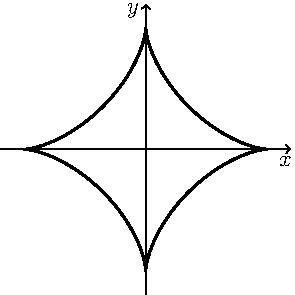
\includegraphics[width=5cm]{./img/Astroid.pdf}
		\caption{Астроида}
		\label{fig:Astroid}
	\end{figure}

	Приступим к решению задачи. Сначала посчитаем ориентированную кривизну по формуле \eqref{eq:OrientedCurvature}. Для этого найдём производные $\dot{\vec{r}}(t)$ (а она уже найдена) и $\ddot{\vec{r}}(t)$:
	\[
		\ddot{\vec{r}}(t) = 3a(2\cos t\sin^2t - \cos^3t, 2\cos^2t\sin t - \sin^3t).
	\]
	Теперь находим ориентированую площадь:
	\begin{multline*}
		S_{\Or}(\dot{\vec{r}}, \ddot{\vec{r}}) = a^2 \cdot \det
		\begin{pmatrix}
			-3\cos^2t\sin t & 3\sin^2t\cos t\\
			2\cos t\sin^2 t - \cos^3t & 2\cos^2t\sin t - \sin^3t
		\end{pmatrix} = \\ = a^2 \cdot (-6\cos^4t\sin^2t + 3\cos^2t\sin^4t - 6\cos^2t\sin^4t + 3\cos^4t\sin^2t) = -3a^2\sin^2t\cos^2t.
	\end{multline*}
	И, наконец, находим ориентированную кривизну:
	\[
		k_{\Or}(t) = \frac{-3a^2\sin^2t\cos^2t}{27a^3\cos^3t\sin^3t} = -\frac{1}{9a\cos t\sin t}.
	\]

	Мы хотим выразить $k_{\Or}$ через натуральный параметр, так что сначала надо найти натуральный параметр:
	\[
		s(t) = \int\limits_0^t\abs{\dot{\vec{r}}(t)}dt = 3a\int\limits_0^t\sin t\cos tdt = \frac{3a}{4}\int\limits_0^t\sin(2t) d(2t) = -\frac{3a}{4}\cos(2t).
	\]
	Итого получаем (здесь уже записываем через радиус кривизны $R = 1 / k$)
	\[
		R^2 = -9a^2\cos^2t\sin^2t = -\frac{9a^2}{4}\sin^2(2t) = \frac{9}{4}\cos^2t - \frac{9a^2}{4} = 4s^2 - \frac{9a^2}{4}.
	\]

	Отметим, что натуральное уравнение не единственное в том смысле, что можно брать натуральный параметр со сдвигом. Здесь, например, немного удобнее взять
	\[
		s(t) = -\frac{3a}{4}\cos(2t) + \frac{3a}{4}.
	\]
	(Это обусловлено тем, что теперь $s(0) = 0$.) Новое уравнение будет выглядеть так:
	\[
		R^2 - 6as - 4s^2 = 0.
	\]
	(Именно в такой форме ответ приведён в задачнике. Алгебраически мы могли его получить просто выделив полный квадрат в старом выражении.)
\end{solution}

В пространстве помимо векторов скорости $\vec{v} \vcentcolon = \dot{\vec{r}}$ и главной нормали $\vec{n} \vcentcolon = \ddot{\vec{r}} / \abs{\ddot{\vec{r}}}$ определяется \textit{вектор бинормали} $\vec{b} \vcentcolon = \vec{v} \times \vec{n}$.

\begin{definition}
	Точку $\vec{r}(s)$ и приложенный к ней базис $(\vec{v}(s), \vec{n}(s), \vec{b}(s))$ называют \textit{репером Френе} пространственной кривой.
\end{definition}

Для этого репера есть аналоги формул \eqref{eq:PlaneFrenet}.

\begin{theorem}[\textit{Формулы Френе для пространственных кривых}]
	Для пространственных кривых выполнено
	\begin{equation} \label{eq:SpaceFrenet}
		\begin{pmatrix}
			\dot{\vec{v}}(s) \\ \dot{\vec{n}}(s) \\ \dot{\vec{b}}(s)
		\end{pmatrix} = 
		\begin{pmatrix}
			0 & k(s) & 0 \\
			-k(s) & 0 & \varkappa(s) \\
			0 & -\varkappa(s) & 0
		\end{pmatrix}
		\begin{pmatrix}
			\vec{v}(s) \\ \vec{n}(s) \\ \vec{b}(s)
		\end{pmatrix},
	\end{equation}
	где $\varkappa(s)$ --- некоторая гладкая функция.
\end{theorem}

\begin{proof}
	Аналогично формулам для плоских кривых, $\dot{\vec{v}} = k\vec{n}$. Из определения, $\abs{\vec{n}} = 1$, значит, $\vec{n} \perp \dot{\vec{n}}$, так что $\dot{\vec{n}} = \alpha\vec{v} + \beta\vec{b}$. Здесь $\alpha = \langle\vec{v}, \dot{\vec{n}}\rangle = -\langle\dot{\vec{v}}, \vec{n}\rangle = -k$, $\beta = \langle\dot{\vec{n}}, \vec{b}\rangle$. $\abs{\vec{b}} = \abs{\vec{v} \times \vec{n}} = 1$, значит, $\dot{\vec{b}} \perp \vec{b}$, отсюда $\dot{\vec{b}} = \alpha\vec{v} + \beta\vec{n}$. Находим коэффициенты: $\alpha = \langle \dot{\vec{b}}, \vec{v} \rangle \hm= -\langle\vec{b}, \dot{\vec{v}}\rangle = 0$, $\beta = \langle\dot{\vec{b}}, \vec{n}\rangle = -\langle \vec{b}, \dot{\vec{n}}\rangle$. Обозначив $\varkappa \vcentcolon = \langle\dot{\vec{n}}, \vec{b}\rangle$, получим формулы \eqref{eq:SpaceFrenet}.
\end{proof}

Геометрический смысл кручения виден из третьего уравнения в \eqref{eq:SpaceFrenet}: это скорость вращения соприкасающейся плоскости кривой в данной точке. Выведем удобную формулу для кручения в натуральной параметризации:
\[
	\dot{\vec{r}} = \vec{v},\quad \ddot{\vec{r}} = \dot{\vec{v}} = k\vec{n},\quad \dddot{\vec{r}} = \frac{d}{ds}(k\vec{n}) = \dot{k}\vec{n} + k\dot{\vec{n}} = \dot{k}\vec{n} - k^2\vec{v} + \varkappa k\vec{b}.
\]
Заметим, что
\[
	\Vol_{\Or}(\dot{\vec{r}}, \ddot{\vec{r}}, \dddot{\vec{r}}) = \Vol_{\Or}(\vec{v}, k\vec{n}, \varkappa k\vec{b}) = k^2\varkappa \underbrace{\Vol_{\Or}(\vec{v}, \vec{n}, \vec{b})}_1 = k^2\varkappa.
\]

Отсюда, $\varkappa(s) = \Vol_{\Or}(\dot{\vec{r}}(s), \ddot{\vec{r}}(s), \dddot{\vec{r}}(s)) / k(s)^2$. Теперь перейдём в произвольную параметризацию. Для этого нужно будет выразить производные по $s$ через производные по $t$, как мы это делали при выводе формулы \eqref{eq:CurvatureFormula}:
\[
	\dot{\vec{r}}(s) = \frac{\vec{r}^\prime(t)}{\abs{\vec{r}^\prime(t)}},\quad \ddot{\vec{r}}(s) = \frac{\vec{r}^{\prime\prime}(t)}{\abs{\vec{r}^\prime(t)}^2}+ \ldots,\quad \dddot{\vec{r}}(s) = \frac{\vec{r}^{\prime\prime\prime}(t)}{\abs{\vec{r}^\prime(t)}^3} + \ldots
\]
Подставляем в формулу для натуральной параметризации:
\begin{multline} \label{eq:TorsionFormula}
	\varkappa(t) = \frac{1}{k^2}\Vol_{\Or}(\dot{\vec{r}}, \ddot{\vec{r}}, \dddot{\vec{r}}) = \frac{\cancel{\abs{\vec{r}^\prime(t)}^6}}{\abs{S_{\Or}(\vec{r}^\prime(t), \vec{r}^{\prime\prime}(t))}} \cdot \frac{1}{\cancel{\abs{\vec{r}^\prime(t)}^6}}\Vol_{\Or}(\vec{r}^\prime(t), \vec{r}^{\prime\prime}(t), \vec{r}^{\prime\prime\prime}(t)) =\\ = \frac{\Vol_{\Or}(\vec{r}^\prime(t), \vec{r}^{\prime\prime}(t), \vec{r}^{\prime\prime\prime}(t))}{\abs{S_{\Or}(\vec{r}^\prime(t), \vec{r}^{\prime\prime}(t))}}.
\end{multline}

Отметим, что из доказательства последней формулы видно, что базис Френе получается из базиса $(\vec{r}^\prime(t), \vec{r}^{\prime\prime}(t), \vec{r}^{\prime\prime\prime}(t))$, который пишется в произвольной параметризации, ортогонализацией Грама "---Шмидта (что, впрочем, верно и в плоском случае).

\begin{proposition}
	Бирегулярная кривая является плоской тогда и только тогда, когда $\varkappa = 0$ (в каждой точке).
\end{proposition}

\begin{proof}
	Легко видеть, что кривая плоская тогда и только тогда, когда $\vec{b}(s) \hm= \vec{v}(s) \times \vec{n}(s) = \const$. Действительно, вектор $\vec{b}$ является просто единичной нормалью плоскости, в которой лежит кривая. А третья формула из \eqref{eq:SpaceFrenet} влечёт, что $\vec{b} = \const$, если и только если $\varkappa = 0$.
\end{proof}

\begin{problem}
	Дана кривая $\vec{r}(t) = (\ch t, \sh t, t)$.
	\begin{enumerate}[nolistsep, label=(\arabic*)]
		\item Привести её к натуральному параметру.
		\item Найти репер Френе в каждой точке.
		\item Найти кривизну и кручение в каждой точке.
	\end{enumerate}
\end{problem}

\begin{solution}
	У этой кривой легко пишутся производные всех порядков:
	\begin{gather*}
		\dot{\vec{r}}(t) = (\sh t, \ch t, 1),\\
		\ddot{\vec{r}}(t) = (\ch t, \sh t, 0),\\
		\dddot{\vec{r}}(t) = (\sh t, \ch t, 0).
	\end{gather*}
	\begin{enumerate}[nolistsep, label=(\arabic*)]
		\item Ищем натуральный параметр по формуле длины кривой:
			\[
				s(t) = \int\limits_0^t\abs{\dot{\vec{r}}(t)}dt = \int\limits_0^t\sqrt{\sh^2t + \ch^2t + 1}dt = \sqrt{2}\int\limits_0^t\ch t\,dt = \sh t\sqrt{2}.
			\]
			Теперь надо каждую координату вектора $\vec{r}(t)$ выразить через натуральный параметр. Для первых двух координат это делается совсем тривиально, а для третьей надо решить квадратное уравнение относительно $e^t$:
			\begin{gather*}
				s = \sqrt{2} \cdot \frac{e^t - e^{-t}}{2},\\
				e^{2t} - s\sqrt{2} \cdot e^t - 1 = 0,\\
				e^t = \frac{s\sqrt{2} + \sqrt{2s^2 + 4}}{2} = \frac{s}{\sqrt{2}} + \sqrt{s^2 + 2},\\
				t = \ln\br{\frac{s}{\sqrt{2}} + \sqrt{s^2 + 2}}.
			\end{gather*}
			Здесь выбрали положительный корень квадратного уравнения, так как $e^t > 0$ для всех $t$. Итого, получаем
			\[
				\vec{r}(s) = \br{\frac{s}{\sqrt{2}}, \sqrt{s^2 + 2}, \ln\br{\frac{s}{\sqrt{2}} + \sqrt{s^2 + 2}}}.
			\]
		\item Воспользуемся ортогонализацией Грама "---Шмидта:
			\[
				\vec{v}(t) = \frac{\dot{\vec{r}}(t)}{\abs{\dot{\vec{r}}(t)}} = \frac{1}{\ch t \sqrt{2}}(\sh t, \ch t, 1) = \frac{1}{\sqrt{2}}\br{\th t, 1, \frac{1}{\ch t}},
			\]
			теперь найдём вектор, совпадающий по направлению с $\vec{n}(t)$:
			\[
				\ddot{\vec{r}}(t) - \frac{\langle \vec{v}(t), \ddot{\vec{r}}(t) \rangle}{\langle \vec{v}(t), \vec{v}(t)\rangle}\vec{v}(t) = (\ch t, \sh t, 0) - \sh t \cancel{\sqrt{2}} \cdot \frac{1}{\cancel{\sqrt{2}}}\br{\th t, 1, \frac{1}{\ch t}} = \br{\frac{1}{\ch t}, 0, -\th t}.
			\]
			Осталось его нормировать, для этого вычислим квадрат его длины:
			\[
				\frac{1}{\ch^2t} + \th^2t = \frac{1 + \sh^2t}{\ch^2t} = 1.
			\]
			Таким образом, нормировать ничего не надо, и $\vec{n}(t) = (1 / \ch t, 0, -\th t)$. Осталось только найти вектор бинормали, это проще делать уже не по Граму "---Шмидту, а просто по определению:
			\[
				\vec{b} = \vec{v} \times \vec{n} = \frac{1}{\sqrt{2}}\det
				\begin{pmatrix}
					\vec{e}_1 & \vec{e}_2 & \vec{e}_3\\
					\th t & 1 & \frac{1}{\ch t}\\
					\frac{1}{\ch t} & 0 & -\th t
				\end{pmatrix} = \frac{1}{\sqrt{2}}\br{-\th t, 1, -\frac{1}{\ch t}}.
			\]
		\item Так как мы уже нашли репер Френе, нам проще не пользоваться формулами \eqref{eq:CurvatureFormula} и \eqref{eq:TorsionFormula} (и тем более не расписывать через натуральный параметр), а исходить из формул Френе. Мы знаем, что $\dot{\vec{v}} = k\vec{n}$, тогда можно просто <<подобрать>> коэффициент пропорциональности между нужными векторами.
			\[
				\dot{\vec{v}}(t) = \frac{1}{\sqrt{2}}\br{\frac{1}{\ch^2t}, 0, -\frac{\sh t}{\ch^2t}} = k(t) \cdot \br{\frac{1}{\ch t}, 0, -\th t}.
			\]
			Отсюда сразу видно, что $k(t) = 1 / (\ch t\sqrt{2})$. Можно так же поступить и для кручения, ведь мы знаем, что $\dot{\vec{b}} = -\varkappa\vec{n}$:
			\[
				\dot{\vec{b}}(t) = \frac{1}{\sqrt{2}}\br{-\frac{1}{\ch^2t}, 0, \frac{\sh t}{\ch^2t}} = -\varkappa(t) \cdot \br{\frac{1}{\ch t}, 0, -\th t}.
			\]
			Получаем $\varkappa(t) = 1 / (\ch t\sqrt{2})$.
	\end{enumerate}
\end{solution}

Решим задачу нахождения кривизны и кручения кривой, которая задана не параметрически, а системой уравнений.

\begin{problem}
	Найти кривизну и кручение кривой, заданной уравнениями
	\[
		\begin{cases}
			x^2 + z^2 - y^2 = 1,\\
			y^2 - 2x + z = 0
		\end{cases}
	\]
	в точке $(1, 1, 1)$.
\end{problem}

\begin{solution}
	Сначала проверим, что в окрестности этой точки пересечение данных поверхностей действительно представляет собой гладкую кривую. Для этого, согласно теореме \ref{theorem:SurfacesToCurve}, достаточно проверить, что точка $(1, 1, 1)$ является регулярной для отображения $\vec{f} = (f_1, f_2)$, где $f_1(x, y, z) = x^2 - y^2 + z^2 - 1$, $f_2(x, y, z) = -2x + y^2 + z$.
	\begin{gather*}
		\left.\nabla f_1\right|_{(1, 1, 1)} = \left.(2x, -2y, 2z)\right|_{(1, 1, 1)} = (2, -2, 2),\\
		\left.\nabla f_2\right|_{(1, 1, 1)} = \left.(-2, 2y, 1)\right|_{(1, 1, 1)} = (-2, 2, 1).
	\end{gather*}

	Видим, что градиенты в интересующих нас точках в самом деле линейно независимы, то есть $\rk J_{\vec{f}}(1, 1, 1) = 2$. Далее мы хотим явно параметризовать данную кривую в окрестности нашей точки. И мы уже знаем, что в качестве параметра нам точно подойдёт какая-то из координат (замечание после доказательства предложения \ref{proposition:SmoothHomeomorphism}), но важно точно понять, какая именно. Нужно посмотреть на матрицу Якоби (которая на самом деле уже выписана сверху) и увидеть два линейно независимых столбца. Подойдут, например, последние два, так что будем выражать переменные $y$ и $z$ через $x$. Целиком выразить $y$ и $z$ из данной нам системы можно, но проблематично. Тем более, позднее мы собираемся пользоваться формулами \eqref{eq:CurvatureFormula} и \eqref{eq:TorsionFormula}, так что нам нужно будет знать их производные вплоть до третьего порядка. Однако можно смотреть на это по-другому --- кроме первых трёх производных нам больше ничего не нужно, так что их и будем искать. Напишем ряды Тейлора с неопределёнными коэффициентами вблизи точки $x = 1$, но чтобы избавиться от обилия возникающих скобок, сделаем замену $\widetilde{x} = x - 1$:
	\begin{gather*}
		y(\widetilde{x}) = 1 + a_1\widetilde{x} + a_2\widetilde{x}^2 + a_3\widetilde{x}^3 + \o(\widetilde{x}^3),\\
		z(\widetilde{x}) = 1 + b_1\widetilde{x} + b_2\widetilde{x}^2 + b_3\widetilde{x}^3 + \o(\widetilde{x}^3).
	\end{gather*}

	Найдём коэффициенты подстановкой в данную нам систему. Для упрощения вычислений можно сложить два уравнения, получив новое уравнение
	\begin{gather*}
		x^2 + z^2 - 2x + z = 1,\\
		\br{x - 1}^2 + \br{z + \frac{1}{2}}^2 - \frac{9}{4} = 0,
	\end{gather*}
	которое связывает $z$ и $x$. В нём надо сделать нашу замену и подставить разложение $z(\widetilde{x})$:
	\begin{gather*}
		\br{z + \frac{1}{2}}^2 = \frac{9}{4} - \widetilde{x}^2,\\
		\br{\frac{3}{2} + b_1\widetilde{x} + b_2\widetilde{x}^2 + b_3\widetilde{x}^3 + \o(\widetilde{x}^3)}^2 = \frac{9}{4} - \widetilde{x}^2.
	\end{gather*}
	
	Раскрываем скобки, отбрасывая члены порядка малости $\o(\widetilde{x}^3)$, и пишем систему на равенство коэффициентов получившихся многочленов в левой и правой части:
	\[
		\begin{cases}
			3b_3 + 2b_1b_2 = 0,\\
			b_1^2 + 3b_2 = -1,\\
			3b_1 = 0.
		\end{cases}
	\]

	Отсюда получаем $b_1 = 0$, $b_2 = -\frac{1}{3}$, $b_3 = 0$. Подставляя, получаем $z(\widetilde{x}) = 1 - \frac{1}{3}\widetilde{x}^2 + \o(\widetilde{x}^3)$. Теперь можем подставить найденное во второе уравнение системы и выразить $y(\widetilde{x})$.
	\begin{gather*}
		\br{1 + a_1\widetilde{x} + a_2\widetilde{x}^2 + a_3\widetilde{x}^3 + \o(\widetilde{x}^3)}^2 - 2(\widetilde{x} + 1) + 1 - \frac{1}{3}\widetilde{x}^2 = 0,\\
		\br{1 + a_1\widetilde{x} + a_2\widetilde{x}^2 + a_3\widetilde{x}^3 + \o(\widetilde{x}^3)}^2 = 1 + 2\widetilde{x} + \frac{1}{3}\widetilde{x}^2.
	\end{gather*}
	Получаем систему:
	\[
		\begin{cases}
			2a_3 + 2a_1a_2 = 0,\\
			a_1^2 + 2a_2 = \frac{1}{3},\\
			2a_1 = 2.
		\end{cases}
	\]

	Отсюда $a_1 = 1$, $a_2 = -\frac{1}{3}$, $a_3 = \frac{1}{3}$. Таким образом, $y(\widetilde{x}) = 1 + \widetilde{x} - \frac{1}{3}\widetilde{x}^2 + \frac{1}{3}\widetilde{x}^3 + \o(\widetilde{x}^3)$. Теперь совершим обратную замену:
	\begin{gather*}
		y(x) = 1 + (x - 1) - \frac{1}{3}(x - 1)^2 + \frac{1}{3}(x - 1)^3 + \o((x - 1)^3),\\
		z(x) = 1 - \frac{1}{3}(x - 1)^2 + \o((x - 1)^3).
	\end{gather*}
	
	Из найденного разложения находим: $y^\prime(1) = 1$, $y^{\prime\prime}(1) = -\frac{1}{3} \cdot 2! = -\frac{2}{3}$, $y^{\prime\prime\prime}(1) = \frac{1}{3} \cdot 3! = 2$ и $z^\prime(1) = 0$, $z^{\prime\prime}(1) = -\frac{1}{3} \cdot 2! = -\frac{2}{3}$, $z^{\prime\prime\prime}(1) = 0$. По формуле кривизны \eqref{eq:CurvatureFormula} имеем
	\[
		k(1) = \frac{\abs{(1, 1, 0) \times (0, -\frac{2}{3}, -\frac{2}{3})}}{\abs{(1, 1, 0)}^3} = \frac{1}{\sqrt{6}}.
	\]
	А по формуле кручения \eqref{eq:TorsionFormula}
	\[
		\varkappa(1) = \frac{\Vol_{\Or}\br{(1, 1, 0), (0, -\frac{2}{3}, -\frac{2}{3}), (0, 2, 0)}}{\abs{(1, 1, 0) \times (0, -\frac{2}{3}, -\frac{2}{3})}^2} = 1.
	\]
\end{solution}

\subsection{Эволюта и эвольвента плоской кривой \label{section:EvoluteInvolute}}

\begin{definition}
	\textit{Эволютой} плоской бирегулярной кривой $\gamma$ называется кривая, которую описывает центр кривизны кривой $\gamma$.
\end{definition}

Пусть $\vec{r}(s)$ --- натуральная параметризация кривой $\gamma$, тогда имеем параметризацию (уже не обязательно натуральную) эволюты:
\begin{equation} \label{eq:Evolute}
	\widetilde{\vec{r}}(s) = \vec{r}(s) + \frac{1}{k(s)}\vec{n}(s).
\end{equation}

\begin{proposition} \label{proposition:NormalEnvelope}
	Кривая $\widetilde{\gamma}$ является эволютой плоской бирегулярной кривой $\gamma$ тогда и только тогда, когда $\widetilde{\gamma}$ является огибающей семейства нормалей к $\gamma$.
\end{proposition}

\begin{proof}
	Пусть $\vec{r}(s)$ --- натуральная параметризация кривой $\gamma$.

	$\Rightarrow$. Параметризация эволюты $\widetilde{\gamma}$ имеет вид \eqref{eq:Evolute}. В каждой точке можем вычислить вектор скорости:\footnotemark
	\[
		\widetilde{\vec{r}}^\prime = \dot{\vec{r}} + \frac{1}{k}\dot{\vec{n}} - \frac{k^\prime}{k^2}\vec{n} = -\frac{k^\prime}{k^2}\vec{n},
	\]
	что и требовалось. (Во втором равенстве воспользовались формулой Френе для плоской кривой $\gamma$.)

	$\Leftarrow$. Можем записать параметризацию $\widetilde{\gamma}$ в виде
	\[
		\widetilde{\vec{r}}(s) = \vec{r}(s) + \lambda(s)\vec{n}(s).
	\]

	Кривая $\widetilde{\gamma}$ является огибающей поля нормалей к $\gamma$. Это значит, что в каждой точке $s$ вектор скорости $\widetilde{\vec{r}}^\prime(s)$ кривой $\widetilde{\gamma}$ должен быть коллинеарен вектору главной нормали $\vec{n}(s)$ кривой $\gamma$, это задаёт условие на коэффициент $\lambda$:
	\[
		\widetilde{\vec{r}}^\prime = (1 - k\lambda)\vec{v} + \lambda^\prime\vec{n}.
	\]
	Отсюда сразу получаем $\lambda = 1 / k$, что и требовалось.
\end{proof}

\footnotetext{Здесь производные берутся по одному и тому же параметру $s$, но обозначены по-разному (точками и штрихами), потому что для кривой $\gamma$ этот параметр натуральный, а для кривой $\widetilde{\gamma}$ --- нет.}

\begin{definition}
	\textit{Эвольвентой} плоской бирегулярной кривой $\gamma$ называется кривая, которую описывает неподвижная точка прямой, катящейся без проскальзывания по $\gamma$.
\end{definition}

Эвольвента (в отличие от эволюты) не определена однозначно, ведь можно выбрать любую точку на катящейся прямой. Так что у бирегулярной плоской кривой имеется однопараметрическое семейство эвольвент. Если $\vec{r}(s)$ --- натуральная параметризация кривой $\gamma$, то легко получить (опять же, необязательно натуральную) параметризацию эвольвенты:
\begin{equation} \label{eq:Involute}
	\widehat{\vec{r}}(s) = \vec{r}(s) - (s - s_0)\dot{\vec{r}}(s).
\end{equation}

Константа $s_0$ как раз соответствует изначальному смещению точки по скользящей прямой, её выбор соответствует выбору эвольвенты.

\begin{theorem}
	Пусть $\gamma$ и $\widehat{\gamma}$ --- регулярные кривые. Следующие условия равносильны:
	\begin{enumerate}[nolistsep, label=(\arabic*)]
		\item кривая $\widehat{\gamma}$ является эвольвентой кривой $\gamma$;
		\item кривая $\gamma$ является огибающей поля нормалей к $\widehat{\gamma}$;
		\item кривая $\gamma$ является эволютой кривой $\widehat{\gamma}$.
	\end{enumerate}
\end{theorem}

\begin{proof}
	Пусть $\vec{r}(s)$ --- регулярная параметризация кривой $\gamma$.

	$(1) \Rightarrow (2)$. Кривая $\widehat{\gamma}$ имеет параметризацию \eqref{eq:Involute}. Вычисляем вектор скорости:
	\[
		\widehat{\vec{r}}^\prime = \cancel{\dot{\vec{r}}} - \cancel{\dot{\vec{r}}} - (s - s_0)\ddot{\vec{r}}
	\]
	и видим, что он перпендикулярен вектору $\dot{\vec{r}}$.

	$(2) \Leftarrow (1)$. Если кривая $\widehat{\gamma}$ ортогональна касательным к $\gamma$, то её параметризация имеет вид $\widehat{\vec{r}}(s) = \vec{r}(s) + \lambda(s)\dot{\vec{r}}(s)$. При этом должно быть выполнено $\langle\widehat{\vec{r}}^\prime, \dot{\vec{r}}\rangle = 0$:
	\[
		0 = \langle (1 + \lambda^\prime)\dot{\vec{r}} + \lambda\ddot{\vec{r}}, \dot{\vec{r}}\rangle = 1 + \lambda^\prime.
	\]
	Отсюда $\lambda(s) = -(s - s_0)$, то есть данная кривая является эвольвентой кривой $\gamma$.

	$(2) \Leftrightarrow (3)$. См. предложение \ref{proposition:NormalEnvelope}.
\end{proof}

\subsection{Дополнительные задачи}

Здесь собраны задачи, которые показались мне интересными, но не вписались в основное повествование. Какие-то из них я умею решать, какие-то нет. Так или иначе, я надеюсь когда-нибудь написать сюда все решения.

\begin{problem}
	Пусть $\vec{r}(s)$ --- натуральная параметризация бирегулярной кривой $\gamma$ в $\R^3$ с ненулевым кручением. Кривая $\gamma$ лежит на сфере тогда и только тогда, когда
	\[
		\frac{\varkappa}{k} = \frac{d}{ds}\br{\frac{dk / ds}{\varkappa k^2}}.
	\]
\end{problem}

\begin{problem}
	Построить гладкую замкнутую плоскую кривую с числом вращения $0$.
\end{problem}

\begin{problem}
	Доказать, что для замкнутой регулярной кривой в $\R^3$ выполняется
	\[
		\oint\limits_{\gamma}k(s)ds \geqslant 2\pi.
	\]
\end{problem}

\begin{problem}
	Пусть $\gamma$ --- гладкая регулярная замкнутая кривая. Доказать, что
	\[
		\oint\limits_{\gamma}(\vec{r}\,dk + \varkappa\vec{b}\,ds) = \vec{0}.
	\]
\end{problem}

\begin{problem}
	\textit{Вершинами} кривой называются точки этой кривой, в которых $k^\prime(s) = 0$. Доказать, что у любой замкнутой регулярной кривой есть по крайней мере четыре вершины.
\end{problem}

\subsection{Про механические часы}

Фраза из эпиграфа связана с историей создания точных механических часов, рассказанной нам Александром Алексадровичем на семинаре.

\textit{Циклоидой} называется кривая, которую описывает неподвижная точка на окружности, движущейся по прямой без проскальзывания.

\begin{figure}[H]
	\centering
	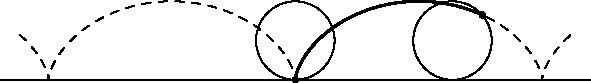
\includegraphics[width=12cm]{./img/Cycloid.pdf}
	\caption{Циклоида}
\end{figure}

В \rnum{17} веке голландский математик\footnotemark{} Х.\,Гюйгенс описал устройство точных механических часов, конструкция которых основана на маятнике, который обладает постоянным периодом качения независимо от амплитуды. Это действительно важное свойство --- период колебания маятника в часах не должен зависеть от силы, с которой заводят часы, или от эффекта постепенного затухания колебаний. Как же может быть устроен такой маятник? Оказывается, конец его нити должен вырисовывать перевёрнутую <<чашу циклоиды>>. Немного позже мы докажем, почему это действительно так, но сейчас зададимся вопросом, как же сделать такой \textit{циклоидный маятник}.

\footnotetext{Гюйгенс, конечно, был не только математиком, но ещё и физиком и философом, что, впрочем, не было исключением для того времени.}

Сначала выведем уравнение циклоиды. Примем за $t = 0$ момент времени, когда точка окружности, движение которой мы отслеживаем, находится на прямой, по которой катится эта окружность. Предположим также, что окружность единичная, а её центр движется равномерно на единицу расстояния за единицу времени. Ясно, что все эти допущения не влияют существенно на уравнения, которые мы будем получать.

\begin{figure}[H]
	\centering
	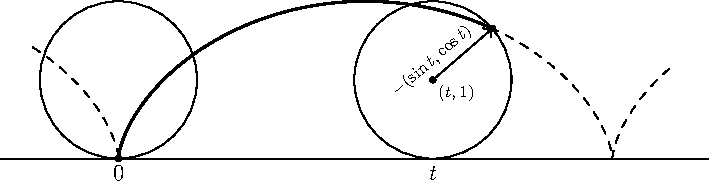
\includegraphics[width=12cm]{./img/CycloidEquation.pdf}
	\caption[format=empty]{}
\end{figure}

Центр окружности в момент времени $t$ находится в точке с координтами $(t, 1)$. Теперь представим, что окружность просто равномерно вращается с закреплённым центром. Тогда движение её граничной точки, конечно, будет описываться вектором $-(\sin t, \cos t)$. Собирая воедино движение центра и точки на границе, получаем искомые координаты в момент времени $t$: $(t - \sin t, 1 - \cos t)$. Однако далее мы всё время будем работать с <<перевёрнутой>> циклоидой, поэтому отразим её относительно горизонтальной прямой:
\[
	\vec{r}(t) = (t - \sin t, \cos t - 1).
\]

\begin{figure}[H]
	\centering
	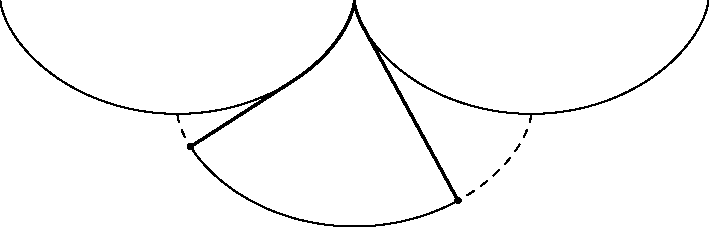
\includegraphics[width=12cm]{./img/Pendulum.pdf}
	\caption{Циклоидный маятник}
	\label{fig:Pendulum}
\end{figure}

Рассмотрим маятник, у которого нить закреплена в вершине между двумя циклоидами (рис. \ref{fig:Pendulum}). Оказывается, свободный конец нити такого маятника будет вырисовывать циклоиду. Ясно, что на самом деле он будет вырисовывать кусок эвольвенты этой циклоиды (просто по определению). Так что утверждение сводится к следующей задаче.

\begin{problem}
	Доказать, что одной из эвольвент циклоиды является конгруэнтная ей циклоида, сдвинутая таким образом, чтобы её <<острия>> перешли в вершины.
\end{problem}

\begin{solution}
	Уравнения эвольвент легко писать, если на исходной кривой введён натуральный параметр. В данном случае это не так, и перейти к натуральному параметру затруднительно. Однако можно заметить, что формулу \eqref{eq:Involute} легко модифицировать и на случай произвольного параметра:
	\[
		\widehat{\vec{r}}(t) = \vec{r}(t) - \frac{\vec{r}^\prime(t)}{\abs{\vec{r}^\prime(t)}}\int\limits_{t_0}^t\abs{\vec{r}^\prime(t)}dt.
	\]

	Действительно, мы просто везде выразили натуральный параметр $s$ через какой-то произвольный параметр $t$. Вычисляем всё, что нужно, положив $t_0 = \pi$ (так обнуляется константа в определённом интеграле).
	\begin{gather*}
		\vec{r}^\prime(t) = (1 - \cos t, -\sin t),\\
		\abs{\vec{r}^\prime(t)}^2 = (1 - \cos t)^2 + \sin^2t = 2(1 - \cos t) = 4\sin^2\frac{t}{2} \Rightarrow \abs{\vec{r}^\prime(t)} = 2\sin\frac{t}{2},\\
		\int\limits_\pi^t 2\sin\frac{t}{2}\,dt = 4\int\limits_\pi^t\sin\frac{t}{2}\,d\br{\frac{t}{2}} = -4\left.\cos\frac{t}{2}\right|_\pi^t = -4\cos\frac{t}{2}.
	\end{gather*}
	А теперь пишем, собственно, уравнение эвольвенты:
	\begin{multline*}
		\widehat{\vec{r}}(t) = (t - \sin t, \cos t - 1) - \frac{\bcancel{2}\br{\sin^{\cancel{2}}\frac{t}{2}, -\cancel{\sin\frac{t}{2}}\cos\frac{t}{2}}}{\bcancel{2} \cdot \cancel{\sin\frac{t}{2}}} \cdot \br{-4\cos\frac{t}{2}} =\\ = (t - \sin t, \cos t - 1) + 2\br{2\sin\frac{t}{2}\cos\frac{t}{2}, -2\cos^2\frac{t}{2}} =\\ = (t - \sin t, \cos t - 1) + (2\sin t, -2 - 2\cos t) = (t + \sin t, -\cos t - 3).
	\end{multline*}
	Итак, получили \[\widehat{\vec{r}}(t) = (t + \sin t, -\cos t - 3) = \big((t + \pi) - \sin(t + \pi), \cos(t + \pi) - 1\big) - (\pi, 2).\]

	Видно, что это сдвинутая циклоида. Легко проверить, что она сдвинута именно так, как указано в условии.
\end{solution}

Теперь мы можем доказать главное утверждение --- что период колебания такого маятника не зависит от амплитуды. Сформулировано оно здесь так же, как в задачнике.

\begin{problem}
	Доказать, что период колебаний материальной точки малой массы, движущейся по чаше перевёрнутой циклоиде без трения в поле силы тяжести, не зависит от её начального положения.
\end{problem}

% TODO: Дописать!

